\begin{frame}{}
    \LARGE Generative AI for Science: \textbf{Chemical Pathways with SMILES}
\end{frame}

\begin{frame}[allowframebreaks]{Chemical Pathways with SMILES}
    \begin{figure}
        \centering
        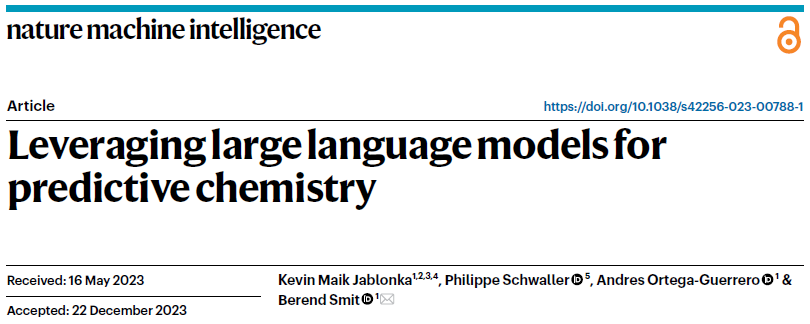
\includegraphics[height=0.9\textheight,width=1\textwidth,keepaspectratio]{images/science/smile-cover.png}
    \end{figure}

    \framebreak

    \begin{figure}
        \centering
        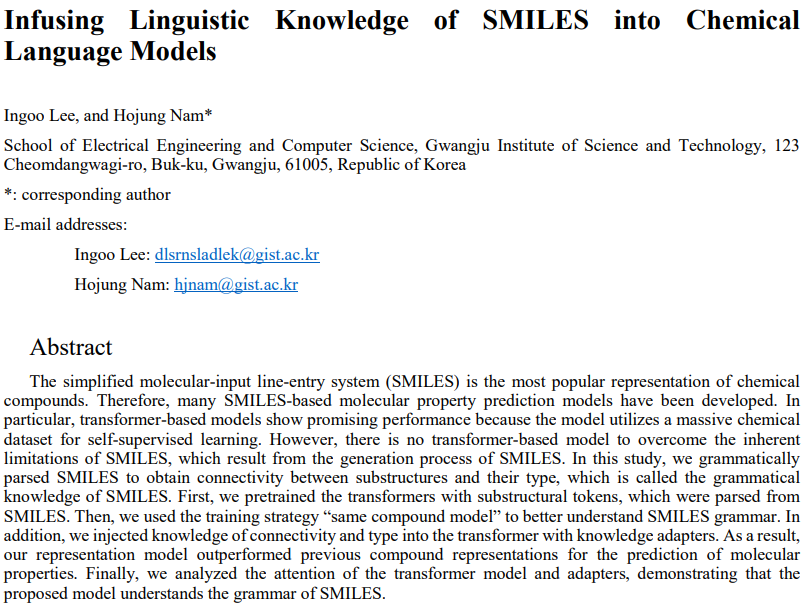
\includegraphics[height=0.9\textheight,width=1\textwidth,keepaspectratio]{images/science/smile-paper.png}
    \end{figure}

    \framebreak
    \textbf{Motivation:}

    \begin{itemize}
        \item Automate synthesis planning to reduce manual effort and errors.
        \item Accelerate chemistry research and development by rapidly exploring chemical pathways.
        \item Enable discovery of novel compounds and efficient reaction routes using generative models.
        \item Leverage SMILES representations for scalable and machine-readable chemistry workflows.
    \end{itemize}

    \framebreak

    \begin{figure}
        \centering
        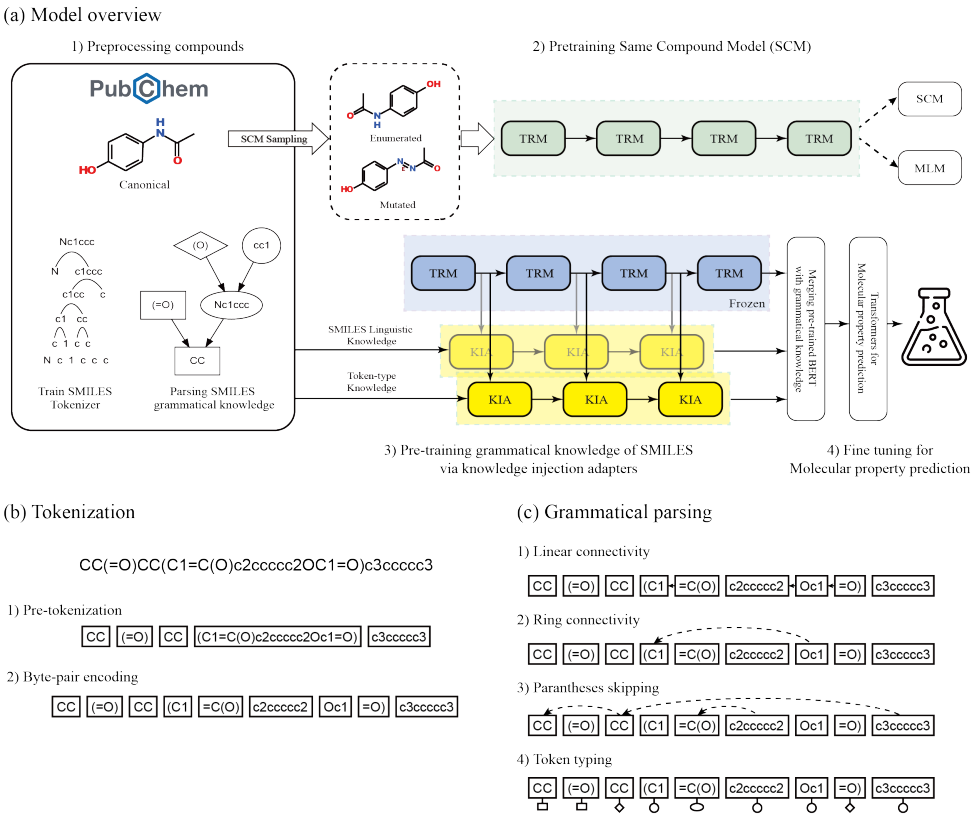
\includegraphics[height=0.9\textheight,width=1\textwidth,keepaspectratio]{images/science/smile-architecture.png}
    \end{figure}

    \framebreak
    \textbf{Key Components:}
    \begin{itemize}
        \item \textbf{SMILES Representation:} A text-based format for encoding chemical structures, enabling easy manipulation and analysis.
        \item \textbf{Generative Models:} AI models that learn from existing chemical data to generate new SMILES strings representing valid chemical compounds.
        \item \textbf{Reaction Prediction:} Models that predict possible reactions and their outcomes based on input SMILES strings.
        \item \textbf{Synthesis Planning:} Algorithms that suggest synthetic routes for target molecules by analyzing reaction networks.
    \end{itemize}

    \framebreak

    \begin{figure}
        \centering
        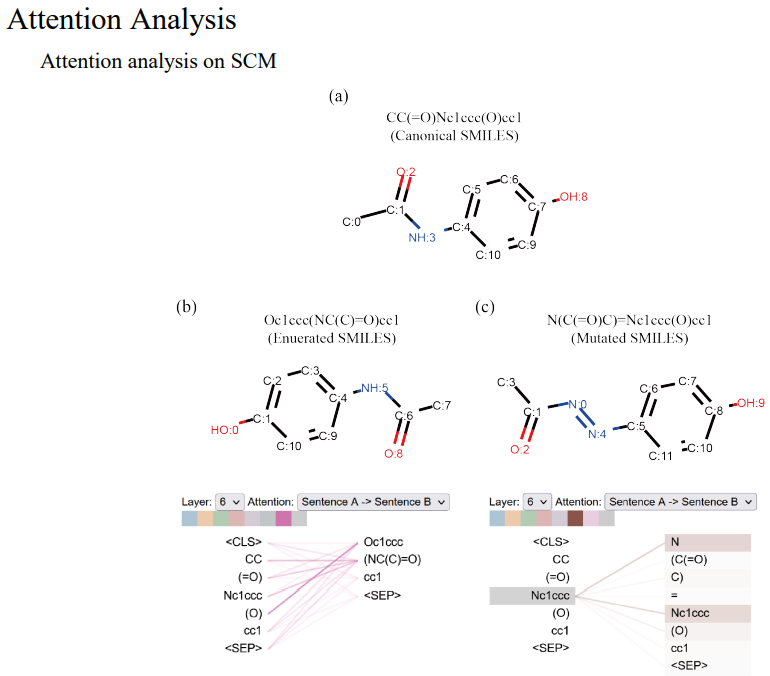
\includegraphics[height=0.9\textheight,width=1\textwidth,keepaspectratio]{images/science/smile-attention.png}
    \end{figure}

    \framebreak
    \textbf{Recent Breakthroughs:}

    \begin{itemize}
        \item \textbf{Leveraging Negative Reactions:} \\
        \href{https://www.science.org/doi/10.1126/sciadv.adk1426}{Science Advances} paper demonstrates that incorporating negative reaction data significantly improves reactivity predictions. \\
        \vspace{0.5em}
        \item \textbf{Emerging Foundation Model: ChemDFM} \\
        Introduction of ChemDFM, a large-scale foundation model for chemistry, enabling broad generalization across chemical tasks. \\
        \href{https://www.cell.com/}{cell.com}
    \end{itemize}

    \framebreak

    \begin{figure}
        \centering
        \href{https://github.com/sanjaradylov/smiles-gpt/blob/master/notebooks/language-modeling.ipynb}{github/sanjaradylov/smiles-gpt}
    \end{figure}

    \framebreak
    \textbf{Limitations:}

    \begin{itemize}
        \item \textbf{Long SMILES Strings (LLD):} Generative models may struggle with very long or complex SMILES representations, leading to invalid or incomplete outputs.
        \item \textbf{Coverage Gaps:} Rare or less-studied chemical reactions and compounds may be underrepresented, limiting the model's ability to generalize.
        \item \textbf{Experimental Validation:} AI-generated pathways and compounds require laboratory validation to confirm feasibility and safety.
    \end{itemize}
\end{frame}